\documentclass[letterpaper,10pt]{IEEEtran}
\usepackage{geometry}                % See geometry.pdf to learn the layout options. There are lots.
\geometry{letterpaper}                   % ... or a4paper or a5paper or ... 
%\geometry{landscape}                % Activate for for rotated page geometry
%\usepackage[parfill]{parskip}    % Activate to begin paragraphs with an empty line rather than an indent
\usepackage{graphicx}
\usepackage{amssymb}
\usepackage{epstopdf}
\usepackage{multicol}
\usepackage{tikz}
\usetikzlibrary{calc}
\usepackage{mathptmx}
\usepackage{amsmath}
\newcommand{\BigO}[1]{\ensuremath{\operatorname{O}\bigl(#1\bigr)}}

\DeclareGraphicsExtensions{.pdf,.png,.jpg}
\usepackage{wrapfig}

% Spacing stuff
\usepackage[cm]{fullpage}
\addtolength{\voffset}{-0.5in}
\setlength{\topmargin}{0pt}
%\setlength\footskip{0pt}
%\setlength{\parskip}{0cm}
%\setlength{\parindent}{1em}
%\usepackage[compact]{titlesec}
%\titlespacing{\section}{0pt}{2ex}{1ex}
%\titlespacing{\subsection}{5pt}{1ex}{2ex}
%\titlespacing{\subsubsection}{0pt}{0.5ex}{0ex}

\title{Mesh Project}
\author{
Donnie Smith (donnie.smith@gatech.edu) \\
Kyle Harrigan (kwharrigan@gatech.edu) 
}	
\date{October 4, 2012}                                           % Activate to display a given date or no date


\markboth{CS 6241 Fall 2012, Project 2}{Shell \MakeLowercase{\text it{et al.}}: A Novel Tin Can Link}
\begin{document}
\maketitle

 \begin{abstract}
 
The initial task of Project 2 was the construction of a Delaunay triangulation of a random set of points using the disk bulge approach and the CLERS labels of the triangles as they are invaded.  An elegant, concise, asnd robust algorithm was implemented as this is desirable for the next phase. A short description of the triangulation approach and of how the corner table (V,S,C) are computed is provided.

Following the construction of the triangulation, the user can to click and drag the mouse to define a polygonal curve that may (partially) overlap the mesh.  As the user is drawing it, the program uses that curve to cut the mesh and should shrink the mesh progressively along the cut to give it a real feeling.
 
 \end{abstract}
 
\section{"Naive" Exhaustive Triangulation}
\IEEEPARstart{I}{nitially} , a naive triangulation algorithm was implemented to produce the Delaunay Triangulation.  This algorithm is a nested loop over all triplets points, looking at all triplet combinations.  For each triplet, it computes the Apollonius circle.  It then loops over all point to determine if they are contained within this circle.  Since this is precisely enforces the condition for the Delaunay triangulation, when it completes it is guaranteed to produce such a triangulation.  The Naive method has complexity of \BigO{n^4} due to the 3 nested loops over vertices and the fourth checking for points.

\section{Bulge Triangulation}
A "bulge" triangulation method was also implemented.  This method is implemented as follows.  The leftmost point is selected as the first vertex (v1).  An imaginary vector pointing directly up is then "swung down" to the right until it encounters the first point.  Mathematically, this is implemented by finding the point which results in the minimum angle between a vector originating at v1 and the vertical and a vector originating at v1 and the test point.  The point which passes this test becomes v2.  
Following this procedure, a recursive bulge process is carried out to the "front" of the segment formed by v1 and v2.     

\section{Corner Table Computation}

\section{Cut Functionality and Logic}

% \includegraphics[width=200px,height=180px]{main/data/physics_init_clipped.png}


\section{Results}
As expected, the bulge triangulation is orders of magnitude faster than the naive implementation.  In the example case shown on this page, for 15 vertices, only 160 calls were made to the Apollonius solver, whereas the naive method required over 455 calls (1.84 times more).  For a larger number of vertices (500), the results are more pronounced: the bulge implementation requires only 249,125 calls and the naive implementation requires 20,708,500 calls (8200 times more).  
The cut functionality works well and provides a real "feeling" as the cut happens. 
\begin{figure}[!t]
\centering
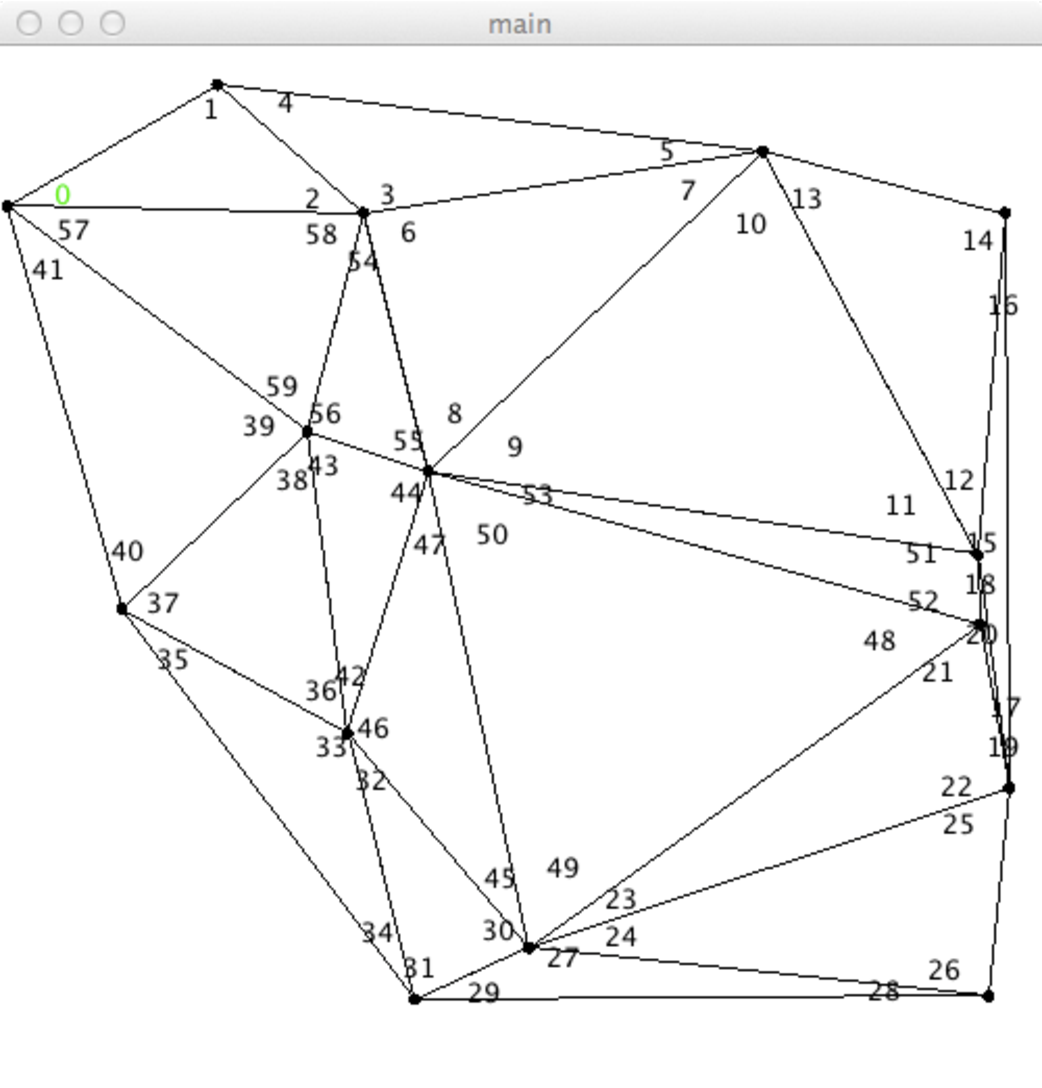
\includegraphics[width=1.75in]{main/data/triangulation}
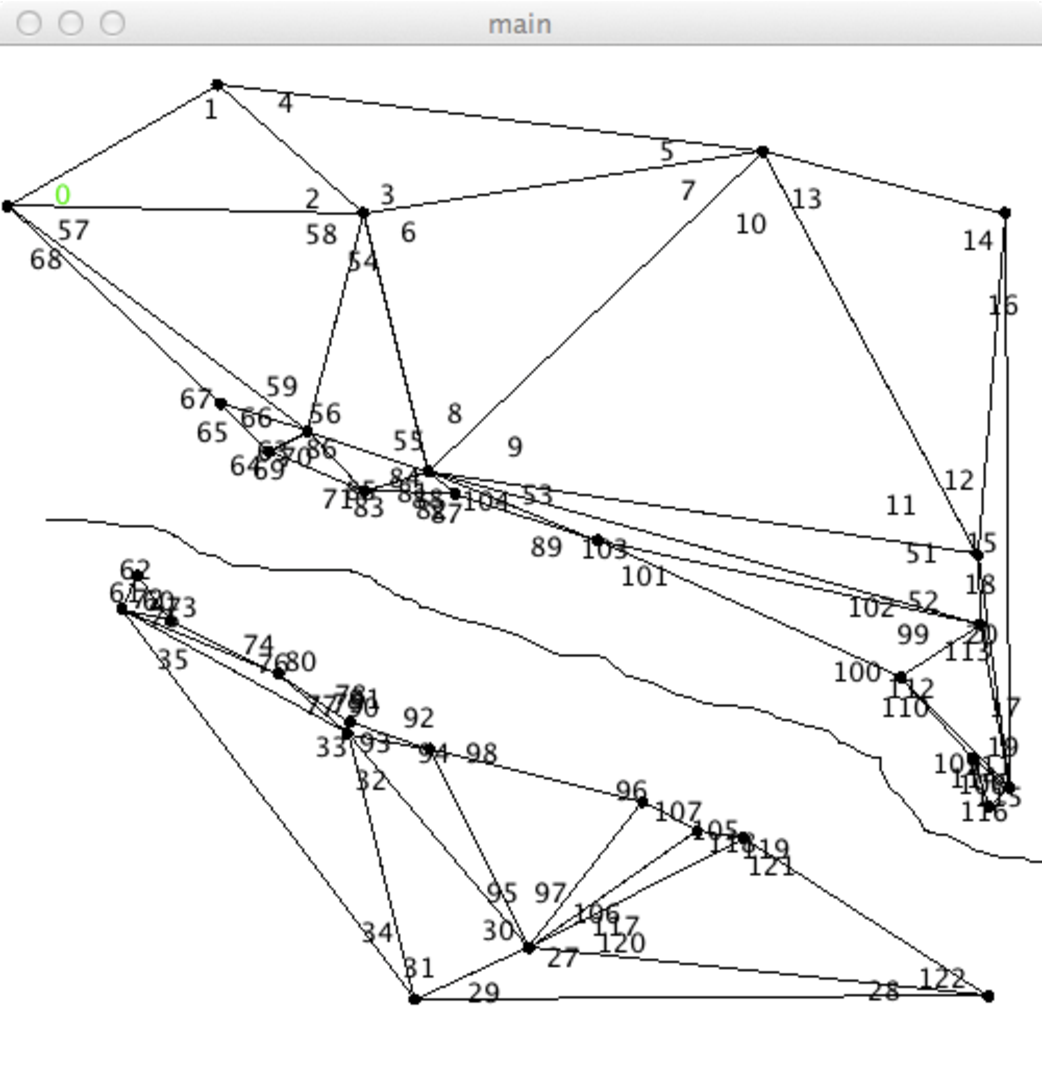
\includegraphics[width=1.75in]{main/data/cut}
\caption{Example Triangulation (left) and a resulting Cut(right)}
\label{fig_triangulation}
\end{figure}

 \section{Future Improvements}
There are numerous improvements that could be made.  The following is a short list we have thought of:

\begin{itemize}
\itemsep0em
\item Improved cut physics by utilizing more complex spring-mass system
\item Implement additional triangulation methods
\item When moving too fast, the cut logic may not function correctly
\end{itemize}
\section{References}
\begin{itemize}
\itemsep0em
\item ...
\end{itemize}

\begin{IEEEbiography}[{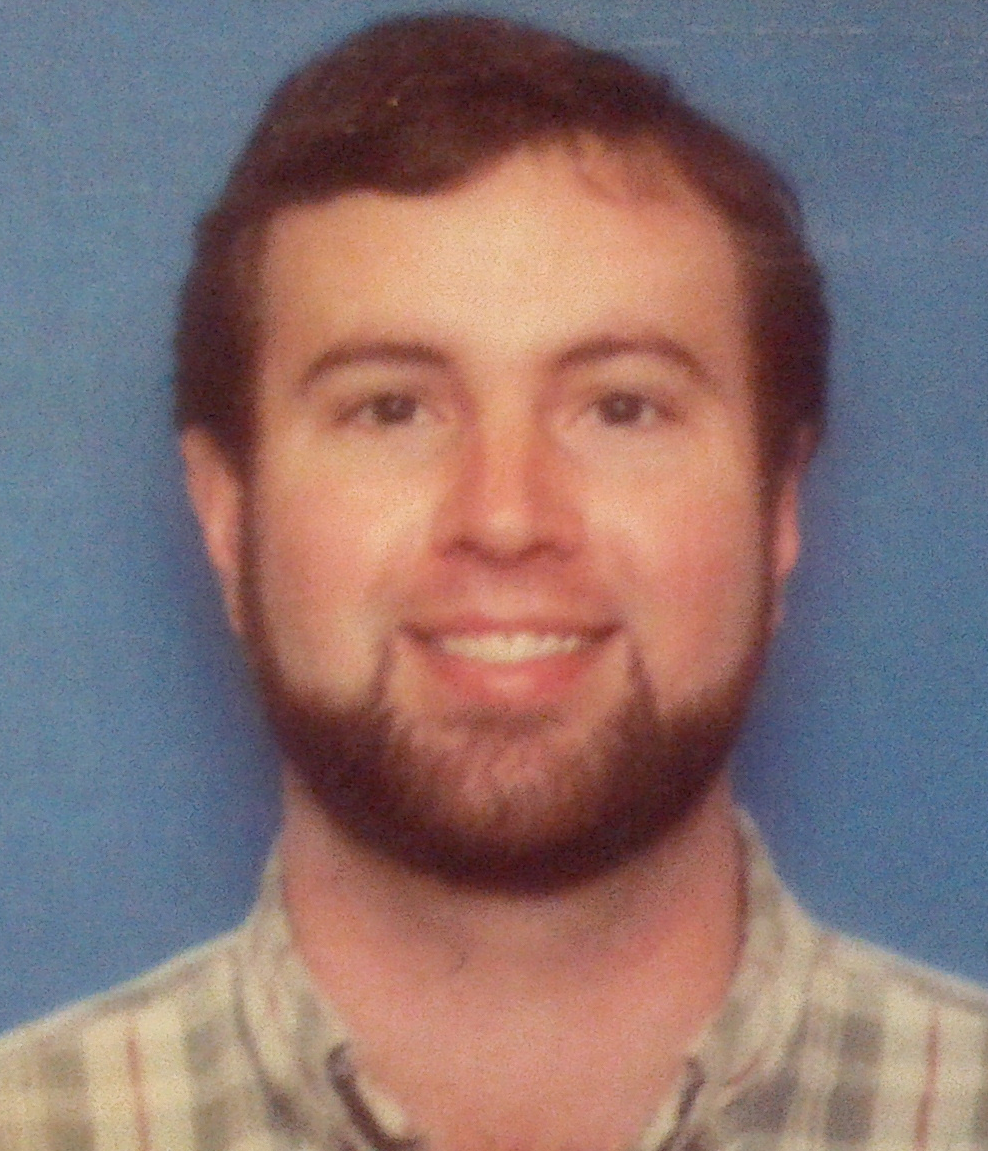
\includegraphics[width=1in,height=1.25in,clip,keepaspectratio]{main/data/dsmith.png}}]{Donnie Smith} 
(M'?)  has been a student of CS 6241 since Fall of 2012.  
\end{IEEEbiography}
\vspace*{-2\baselineskip}
\begin{IEEEbiography}[{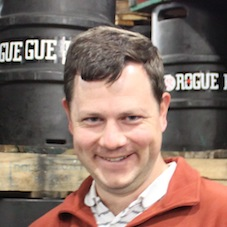
\includegraphics[width=1in,height=1.25in,clip,keepaspectratio]{main/data/kwharrigan.jpg}}]{Kyle Harrigan} 
(M'?) has been a student of CS 6241 since Fall of 2012.  
\end{IEEEbiography}

\end{document}  



